% !TEX root = ../beamer.tex

\begin{frame}[fragile, plain]
	\plainnumber
	\frametitle{Workflow Specification}
	
	\begin{minipage}{0.45\textwidth}
	    		        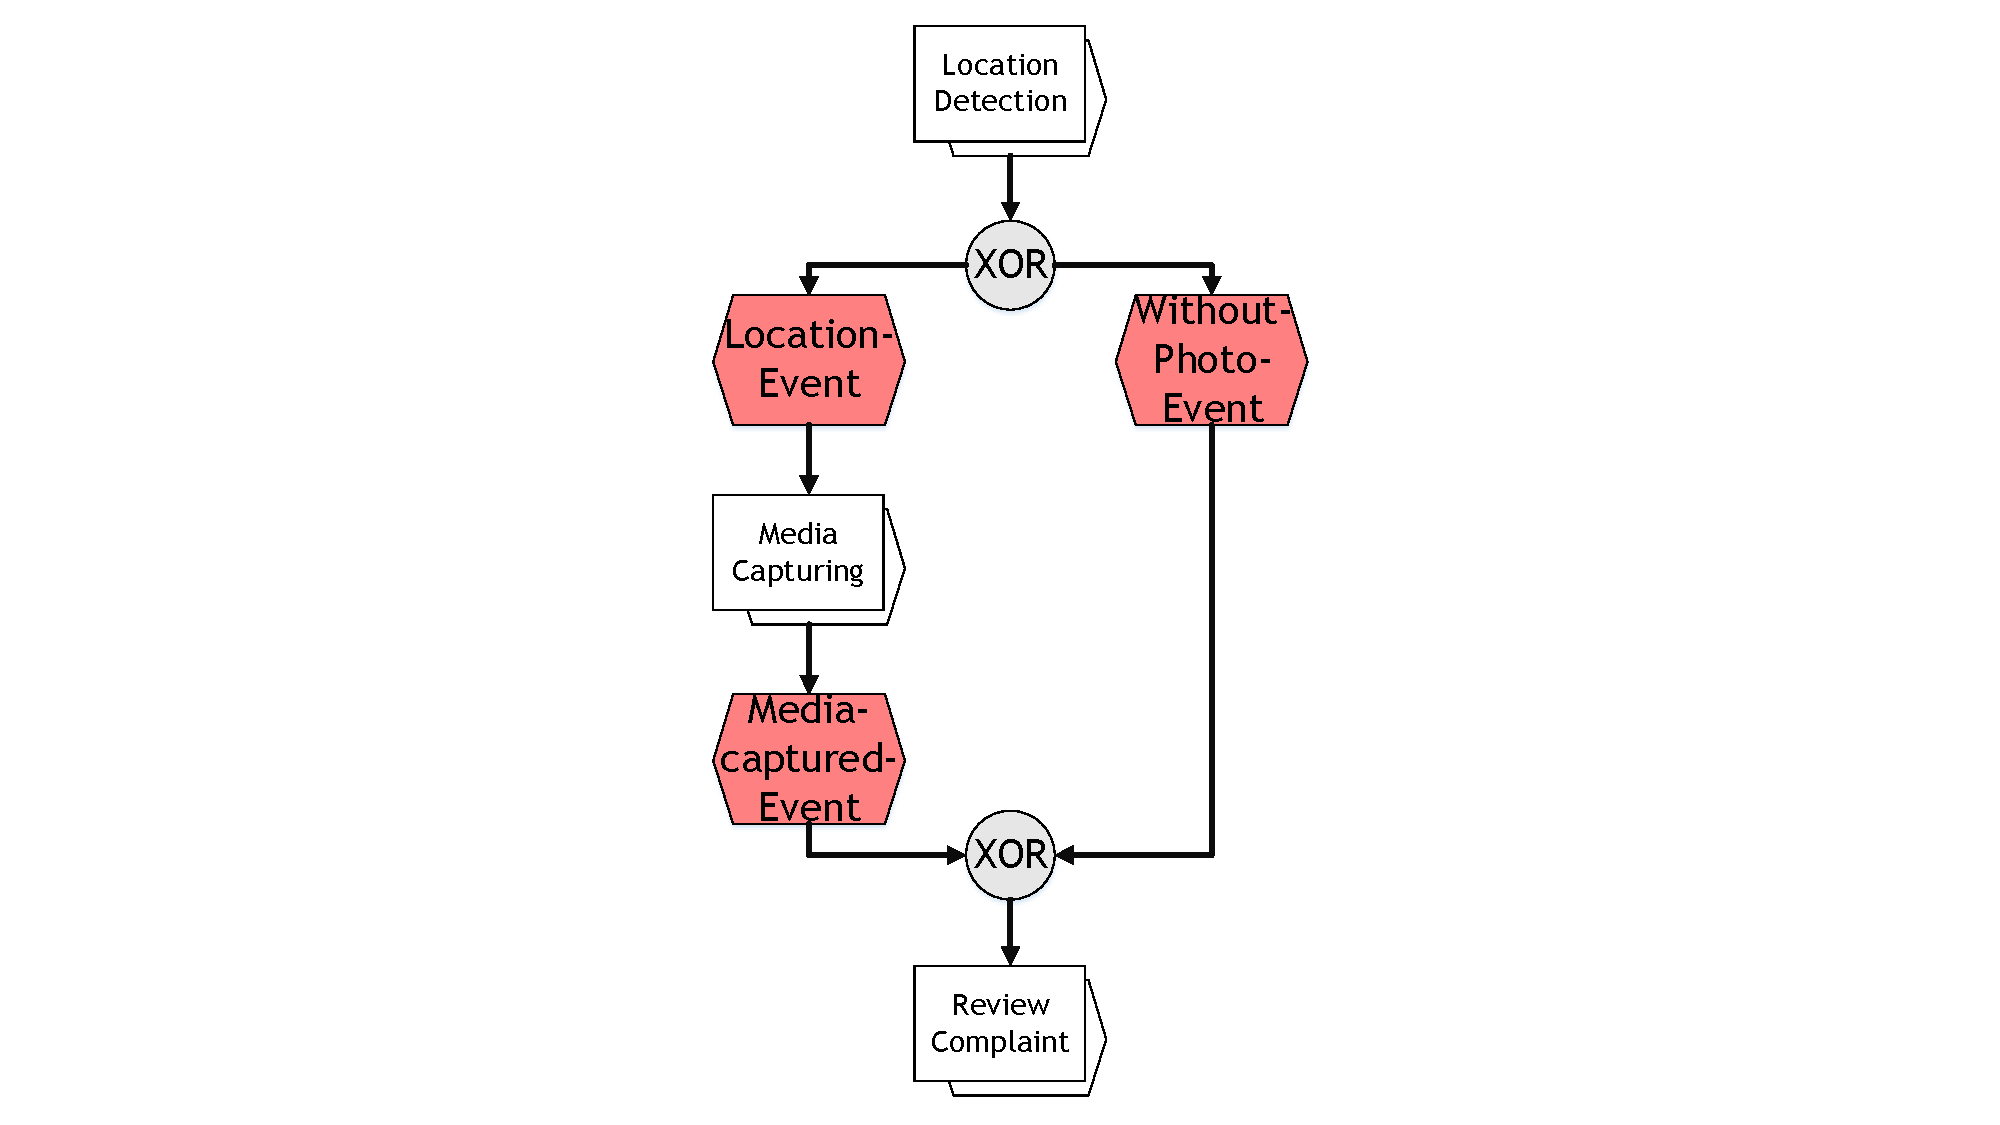
\includegraphics[height = 7cm, trim = 10cm 0cm 10cm 0cm, clip = true]{images/WorkflowSpecification.pdf}	  
	\end{minipage}\hfill
	\begin{minipage}{0.5\textwidth}
\begin{lstlisting}
WorkflowElement LocationDetection
  fires LocationEvent {
    start Mediacapturing
  }
  fires WithoutPhotoEvent {
    start SubmitComplaint
  }

WorkflowElement MediaCapturing
  fires MediacapturedEvent {
    start SubmitComplaint
  }

App CitizenApp {
  WorkflowElements {
    LocationDetection (startable: "Start Complaint"),
    MediaCapturing,
    ...
  }
}
\end{lstlisting}
\end{minipage}

\end{frame}

\begin{frame}[fragile]
	\frametitle{Calling external Webservices}
	\begin{lstlisting}[basicstyle=\footnotesize]
	externalWebService sendEmail {
	   url "http://psmd2.uni-muenster.de:8080/SendMail/api/mail/send/"
	   method GET
	   queryparams (
	     "to" : "md2@trashmail.de"
	     "subject" : "Map.Apps E-Mail"
	     "body" : "Dear ladies and gentlemen, this is an e-mail sent by md2 map.apps!"
	   )
	}
	
	bind action WebServiceCall sendEmail on EmailView.SendButton.onClick
	\end{lstlisting}
\end{frame}

\begin{frame}[fragile]
	\frametitle{Starting Workflows from external WS Calls}
	\begin{lstlisting}[basicstyle=\footnotesize]
	WorkflowElement LocationDetection (invokable)
	  fires ...
		
	invokable at "address" using POST {
			set :ComplaintProvider.loc to :AddressProvider
			:AddressProvider.myStreet
			:AddressProvider.myStreetNo
			:AddressProvider.myCity
			:AddressProvider.myPostalCode
			default :ComplaintProvider.status = "User is filling out complaint" 
		}
	\end{lstlisting}
\end{frame}

\begin{frame}[t]
    \frametitle{DSL}
\end{frame}

\begin{frame}[t]
    \frametitle{Generated Code}
\end{frame}

\begin{frame}[t]
    \frametitle{Generator}
    
	\begin{center}   
	\begin{tikzpicture}[
		>=stealth,
		node distance = 0.75cm and 0.25cm,
		every node/.style={minimum height = 1.75em}]
		\node[draw] (dsl) {DSL\vphantom{Aq}};
		\node[draw, below = of dsl] (md2model) {\MD Model\vphantom{Aq}};
		\draw[->] (md2model) -- node[right] {\tiny{uses}} (dsl);
	    
		\node[below = of md2model, draw] (preprocessor) {Preprocessor\vphantom{Aq}};
		\draw[->] (md2model) -- node[right] {\tiny{processed by}} (preprocessor);
		
		\node[draw, below = of preprocessor] (generator) {Generator\vphantom{Aq}};
		
		\draw[->] (preprocessor) -- node[right] {\tiny{input for}} (generator);
		
		\node[draw, below left = 0.25cm of generator] (mapapps) {map.apps source\vphantom{Aq}};
		\node[draw, below right = 0.25cm of generator] (backend) {backend source\vphantom{Aq}};
		
		\draw[->] (generator) -| node[above] {\tiny{generates}} (mapapps);
		\draw[->] (generator) -| node[above] {\tiny{generates}} (backend);
	\end{tikzpicture}
	\end{center}
\end{frame}

\begin{frame}
    \frametitle{Deployment}
    
    \begin{center}   
	    \begin{tikzpicture}[
	    >=stealth,
	    node distance = 0.75cm and 0.25cm,
	    big/.style = {draw, minimum width = 2.5cm, minimum height = 1.75em}
	    ]
	    \node[big] (generator) {Generator};
	    \node[big, below left = of generator] (mapapps) {map.apps source\vphantom{Aq}};
	    \node[big, below right = of generator] (backend) {backend source\vphantom{Aq}};
	    \draw[->] (generator) -| node[above] {\tiny{generates}} (mapapps);
	    \draw[->] (generator) -| node[above] {\tiny{generates}} (backend);
	    \node[big, rounded corners, below = of mapapps] (jetty) {Jetty\vphantom{Aq}};
	    \node[big, rounded corners, below = of backend] (glassfish) {Glassfish\vphantom{Aq}};
	    \draw[->] (mapapps) -- node[left] {\tiny{deployed on}} (jetty);
	    \draw[->] (backend) -- node[right] {\tiny{deployed on}} (glassfish);
	    \draw[<->] (jetty) -- node[above] (communicates) {\tiny{communicates}} (glassfish);
	    
	    \node[big, rounded corners, below = of communicates] (tomcat) {Tomcat};
	    \node[big, gray, below = 0cm of tomcat] {map.apps full};	    
	    
	    \end{tikzpicture}
    \end{center}
\end{frame}

